% !TeX root = ../tesis.tex

\section{Reflectancia y transmitancia de una monocapa de nanopartículas de materiales reales: oro y plata}
\label{section:AuAg}

Con la finalidad de presentar la respuesta óptica de una monocapa de NPs esféricas hechas con materiales realista, se emplea en esta sección la función dieléctrica con corrección por tamaño para NPs esféricas de oro [Fig. \ref{sfig:sizeAu}] y de plata [Fig. \ref{sfig:sizeAg}]. La elección de NPs de oro y plata surge a partir del uso frecuente de estos materiales para el biosensado \cite{jain2008noble,estevez2014trends}, así como por su biocompatibilidad \cite{fan2009bio,bosetti2002silver}. Se realizaron cálculos de la reflectancia en configuración ATR para monocapas de NPs esféricas de oro y monocapas de NPs esféricas de plata dado que en este esquema, para NPs con una función dieléctrica descrita por el modelo de Drude [Ec. \eqref{eq:Drude}], se identificó un supuesto modo plasmónico colectivo el cual, si se presenta también en materiales reales, podría usarse en biosensado. De forma análoga a la sección \ref{ssection:DrudeATR}, se presentan cálculos de la reflectancia  considerando monocapas conformadas por NPs tanto de oro como de plata, variando los parámetros $\Theta$ (fracción de cubierta) y  $a$ (radio de las NPs) para identificar y caracterizar al supuesto modo plasmónico colectivo, así como para optimizar estos parámetros para el biosensado. Adicionalmente, se calcula la transmitancia de las monocapas de NPs de oro y de plata para corroborar que el supuesto modo plasmónico colectivo presenta características de un modo guiado, como se observó para una monocapa de NPs con una función dieléctrica tipo Drude.

En la Fig.  \ref{fig:Au-R-Theta} se muestran los cálculos de la reflectancia $R$, empleando el CSM, de una monocapa de NPs esféricas idénticas de oro con un radio de $a = 25$ nm, inmersa en una matriz de agua ($n_m = 1.33$) y soportada por un sustrato con un índice de refracción $n_s = 1.5$, que es iluminada por una onda plana en una configuración ATR. La reflectancia se grafica como función del ángulo de incidencia $\theta_i$ y tanto de la longitud de onda $\lambda$ (escala inferior), como de la energía en unidades de $\hbar\omega$ (escala superior). Se consideraron las fracciones de cubierta $\Theta = 0.1,\,0.125,\,0.15,\, 0.175$ y $0.2$ ---garantizando las condiciones de validez del CSM---, así como la polarización de la onda plana incidente: las gráficas \textbf{i)}--\textbf{v)} corresponden a la polarización \emph{p} y \textbf{vi)}--\textbf{x)} a \emph{s}. Las líneas punteadas verticales verdes y rosas corresponden a las SP-SPRs dipolares y cuadrupolares, respectivamente: para una NP de oro de $a= 25$ nm inmersa en agua, la SP-SPR dipolar se localiza en $\lambda \approx 531$ nm y la cuadrupolar en $513$ nm. Los puntos amarillos, localizados a longitudes de onda mayores a las de la SP-SPR dipolar, corresponden al supuesto modo plasmónico colectivo. A diferencia de los cálculos de la reflectacia de una monocapa de NPs  con una función dieléctrica tipo Drude analizada en la sección \ref{ssection:DrudeATR}, para una monocapa de NPs de oro se observan las contribuciones no plasmónicas de la función dieléctrica del oro para $\lambda<513$ nm. Sin embargo, dado que el supuesto modo plasmónico colectivo se excita a energías menores a las  SP-SPRs, la contribución de los electrones ligados no se traslapa con el supuesto modo plasmónico colectivo. 

	\begin{figure}[t!]\centering
\hspace*{-.5em}\begin{tikzpicture}[scale=1]
\node[inner sep=0pt] (graf) at (-.15,0){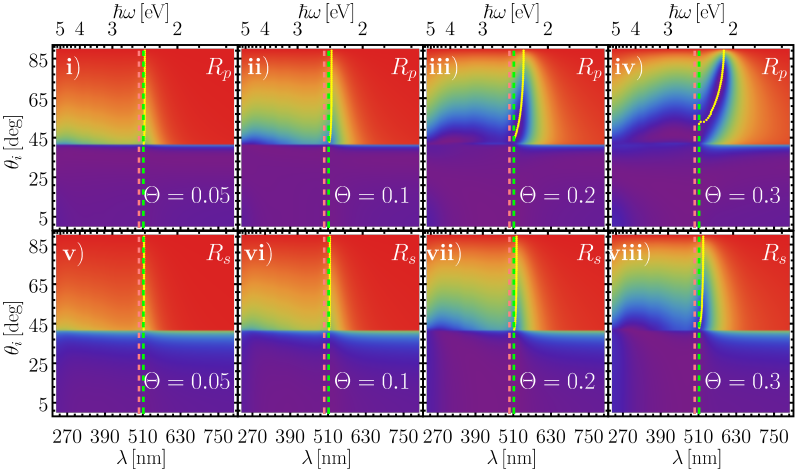
\includegraphics[scale=1]{2-Resultados/figs/6-AuThetaVar/0-2D_Grid}};
\node[right, inner sep=0pt] (legend) at (7.1,.15) {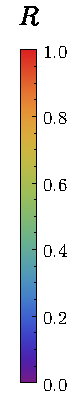
\includegraphics[scale=1, trim={00 -15 00 00}, clip]{2-Resultados/figs/0-RBar_v}};

\def\y{4.2}
	\node at(-5.2,\y){\normalsize $\Theta = 0.10 $};
	\node at(-2.4,\y){\normalsize $\Theta = 0.125 $};
	\node at(0.4,\y) {\normalsize $\Theta = 0.15$};
	\node at(3.2,\y) {\normalsize $\Theta = 0.175 $};
	\node at(6.0,\y) {\normalsize $\Theta = 0.2 $};

\def\xR{6.8}
\def\yR{2.4}	
	\node at(\xR,\yR){$R_p $};
	\node at(\xR,\yR-2.8){$R_s$};
\end{tikzpicture}\vspace*{-.5em}	
	\caption{Gráficas de la reflectancia en configuración ATR  de una monocapa de NPs esféricas de oro de radio $a=25$ nm como función del ángulo de incidencia $\theta_i$ y de la longitud de onda $\lambda$ (escala inferior), así como de la energía de la onda plana incidente en unidades de $\hbar\omega$ (escala superior).  Las gráficas   en el renglón superior [\textbf{i)--v)}] muestran los resultados para  polarización \emph{p} y las del renglón inferior  [\textbf{vi)}--\textbf{x)}]  para polarización  \emph{s}, donde se consideraron los valores de fracción de cubierta $\Theta =  0.1,\,0.125,\,0.15,\, 0.175$ y $0.2$.  Las líneas verticales punteadas verdes y rosas corresponden a las SP-SPRs dipolar en $\lambda=531$ nm y  cuadrupolar en $\lambda=513$ nm, respectivamente.  Los puntos amarillos corresponden a los mínimos en $R$ para ángulos mayores a $\theta_c\approx 62.5^\circ$ y longitudes de onda mayores a la SP-SPRs dipolar.
}	\label{fig:Au-R-Theta}	
	\end{figure}	

En la Fig.  \ref{fig:Au-R-Theta}, en las gráficas \textbf{i)}, \textbf{ii)}, \textbf{vi)} y \textbf{vii)}, correspondientes a $\Theta=0.1$ y $0.125$ para ambas polarizaciones, el supuesto modo plasmónico colectivo se excita a valores de $\lambda$ cercanos a la SP-SPR dipolar para ángulos de incidencia alrededor del ángulo crítico $\theta_c$. Sin embargo para valores de $\Theta\geq 0.175$, no es apreciable ningún mínimo en la reflectancia para $\theta_i\approx\theta_c$; por ejemplo para $\Theta=0.2$ para polarización \emph{p} [gráfica \textbf{v)}] a $\lambda = 531$ nm (línea punteada vertical verde) el supuesto modo plasmónico colectivo (puntos amarillos) se excita a partir de $\theta\approx 75^\circ$, mientras que para \emph{s} [gráfica \textbf{x)}] a partir de $\theta_i\approx 65^\circ$. Es decir, a diferencia de los resultados obtenidos al emplear el modelo de Drude para la función dieléctrica de las NPs en la monocapa, el supuesto modo plasmónico colectivo en una monocapa de NPs de oro no puede excitarse a todos los ángulos de incidencia a menos que $\Theta\leq 0.15$. Al comparar la respuesta EM de la monocapa para las dos polarizaciones, el corrimiento al rojo del supuesto modo plasmónico colectivo respecto a la SP-SPR dipolar es mayor  para polarización \emph{p}, \textbf{v)}, que para \emph{s}, \textbf{x)} ---comportamiento también observado al considerar una respuesta tipo Drude para las NPs de la monocapa---.

La reflectancia de una monocapa de NPs con las mismas características que las de la Fig. \ref{fig:Au-R-Theta} pero con NPs esféricas de plata, de radio $a=35$ nm, se grafica en la Fig. \ref{fig:Ag-R-Theta}. El radio de las NPs de plata se eligió mayor que el de las NPs de oro para sintonizar la SP-SPR dipolar (líneas verticales verdes) en el espectro visible en $\lambda=430$ nm; la SP-SPR cuadrupolar (líneas verticales rosas) se sintoniza en $\lambda=375$ nm. Al igual que para la función dieléctrica del oro, la de la plata cuenta con contribuciones no plasmónicas mas éstas no pueden ser excitadas en el espectro visible, por lo que los cálculos de la reflectancia de una monocapa de NPs de plata se asemejan a los resultados obtenidos al considerar el modelo de Drude-Sommerfeld, como se observa al comparar las Figs. \ref{fig:R-ATR4} (modelo de Drude-Sommerfeld con $\hbar\omega_p=4.3$ eV) y \ref{fig:Ag-R-Theta} (NPs de plata).

\begin{figure}[h!]\centering
\hspace*{-.5em}\begin{tikzpicture}[scale=1]
\node[inner sep=0pt] (graf) at (-.15,0){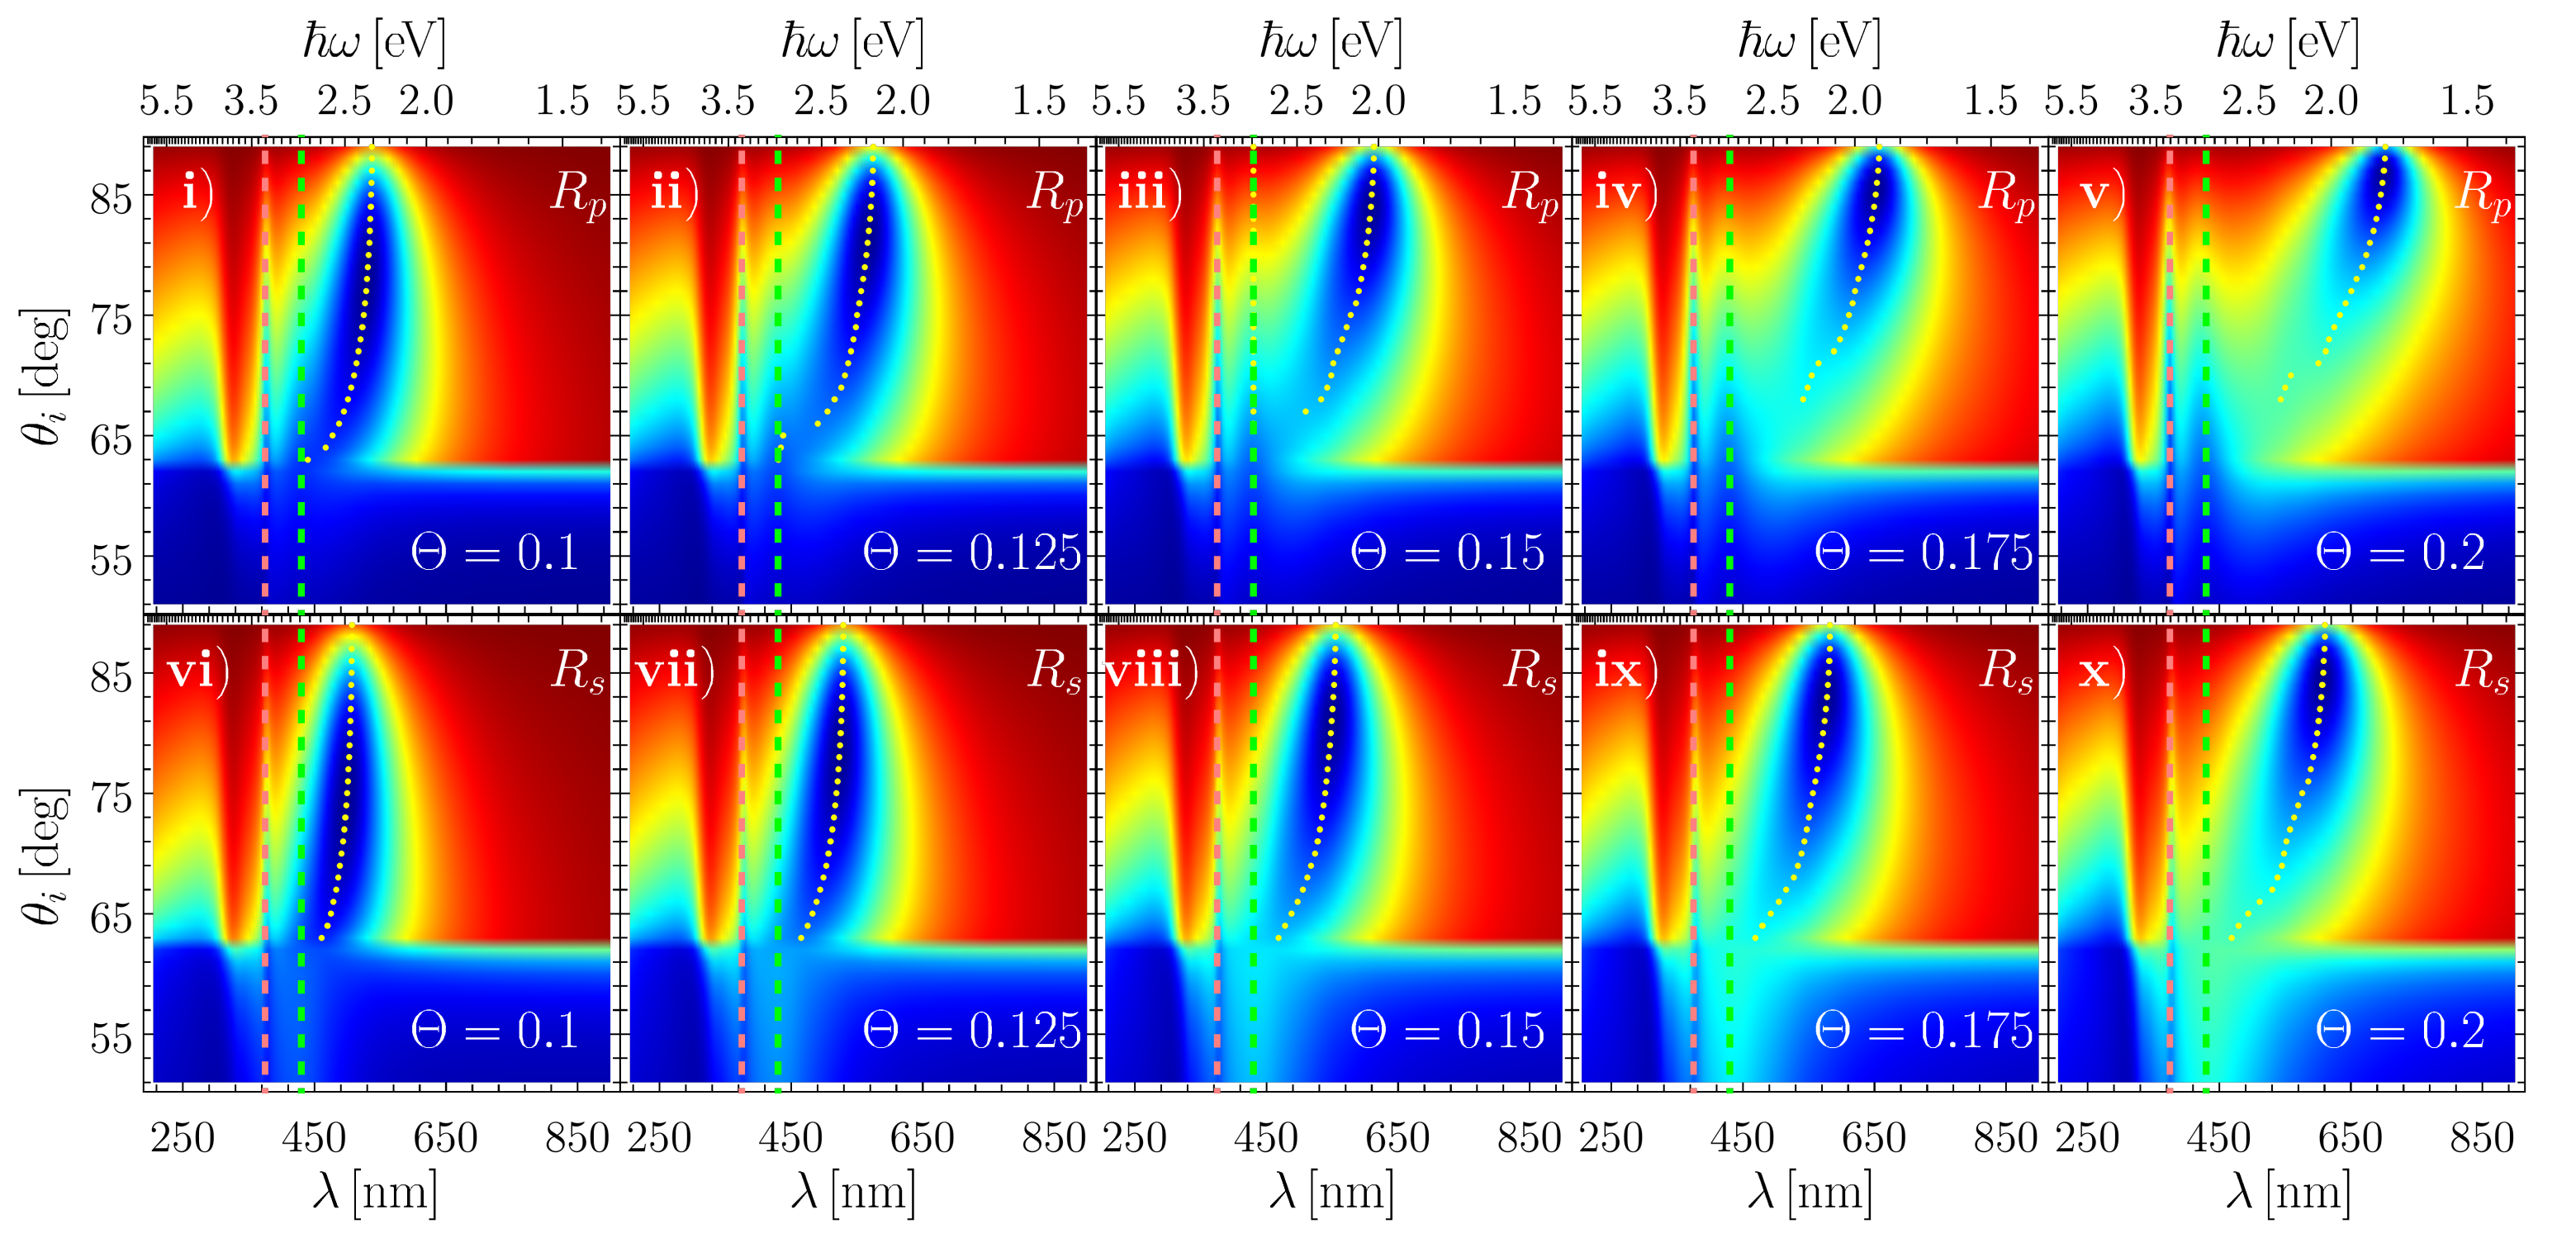
\includegraphics[scale=1]{2-Resultados/figs/7-AgThetaVar/0-2D_Grid}};
\node[right, inner sep=0pt] (legend) at (7.1,.15) {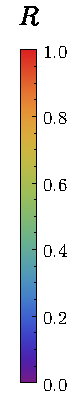
\includegraphics[scale=1, trim={00 -15 00 00}, clip]{2-Resultados/figs/0-RBar_v}};

\def\y{4.2}
	\node at(-5.2,\y){\normalsize $\Theta = 0.10 $};
	\node at(-2.4,\y){\normalsize $\Theta = 0.125 $};
	\node at(0.4,\y) {\normalsize $\Theta = 0.15$};
	\node at(3.2,\y) {\normalsize $\Theta = 0.175 $};
	\node at(6.0,\y) {\normalsize $\Theta = 0.2 $};

\def\xR{6.8}
\def\yR{2.4}	
	\node at(\xR,\yR){$R_p $};
	\node at(\xR,\yR-2.8){$R_s$};
\end{tikzpicture}\vspace*{-.5em}
	\caption{Gráficas de la reflectancia de una monocapa de NPs esféricas de plata de radio $a=35$ nm en configuración ATR como función del ángulo de incidencia $\theta_i$ y de la longitud de onda $\lambda$ (escala inferior), así como de la energía de la onda plana incidente en unidades de $\hbar\omega$ (escala superior).  Las gráficas   en el renglón superior [\textbf{i)--v)}] muestran los resultados para  polarización \emph{p} y las del renglón inferior  [\textbf{vi)}--\textbf{x)}]  para polarización  \emph{s}, donde se consideraron los valores de fracción de cubierta $\Theta = 0.1,\,0.125,\,0.15,\, 0.175$ y $0.2$.  Las líneas verticales punteadas verdes y rosas corresponden a las SP-SPRs dipolar en $\lambda=430$ nm y  cuadrupolar en $\lambda=375$ nm, respectivamente.  Los puntos amarillos corresponden a los mínimos en $R$ para ángulos mayores a $\theta_c\approx 62.5^\circ$ y longitudes de onda mayores a la SP-SPRs dipolar.
}	\label{fig:Ag-R-Theta}	
	\end{figure}	

En la reflectancia para la monocapa de NPs de plata, Fig. \ref{fig:Ag-R-Theta}, la SP-SPR cuadrupolar (línea vertical punteada rosa) se aprecia a $\lambda\approx 375$ nm para todos los valores de $\Theta$ considerados, sin embargo, la SP-SPR dipolar (línea punteada vertical verde) sólo se aprecia para polarización \emph{p} cuando $\Theta=0.2$, gráfica \textbf{v)}, mientras que para \emph{s} no se aprecia para ningún valor de $\Theta$, característica también observada para las NPs con una función dieléctrica tipo Drude en la Fig. \ref{fig:R-RVar}. Otra semejanza entre los resultados obtenidos con el modelo de Drude-Sommerfeld y con las NPs de plata, pero que no se observa con las NPs de oro, es el límite del supuesto modo plasmónico colectivo cuando $\theta_i$ tiende a $\theta_c$, en donde la longitud de onda de excitación del supuesto modo plasmónico colectivo tiende a la SP-SPR dipolar.

Tanto para la monocapa de NPs de oro, como de NPs de plata, la reflectancia a las longitudes de onda del supuesto modo plasmónico colectivo (puntos amarillos en las Figs. \ref{fig:Au-R-Theta} y \ref{fig:Ag-R-Theta}) para  $\Theta\geq 0.175$ es mínima a ángulos de incidencia rasantes ($\theta_i\lessapprox 90^\circ$) y los valores de $\theta_i$ donde $R$ es mínima disminuyen conforme $\Theta$ decrece.  Adicionalmente, el ancho de la resonancia a ángulos rasantes (para oro y plata) es menor en comparación al resto de los ángulos por lo que podría proponerse para ser usado en el biosensado. Sin embargo para ángulos grandes, en la medición experimental de la reflectancia, el área del haz de luz incidente se deforma (extiende) al incidir sobre la interfaz entre el sustrato y la matriz mediante la transformación $A\to A'/\cos\theta_i$, en donde $A$ es el área del haz al incidir sobre la interfaz  y $A'$ es la sección transversal del haz (ver Fig. \ref{fig:hazcircular}). La deformación del haz complica las mediciones de reflectancia a incidencia rasante, restringiendo el valor de $\theta_i$ a ángulos menores a $80^\circ$, valor para el que el diámetro del haz, en la dirección paralela a la interfaz, aumenta en un factor de $5.7$.

Una diferencia entre los resultados de la reflectancia de las monocapas de NPs de oro y plata, es el valor de $\theta_i$ al cual se comienza a excitar el supuesto modo plasmónico colectivo una vez escogido $\Theta$. Para analizar este comportamiento, se grafican en la Fig. \ref{fig:AuAg-Cuts-65} cortes de la reflectancia graficada en las Figs. \ref{fig:Au-R-Theta} (para las NPs de oro) y \ref{fig:Ag-R-Theta} (para las NPs de plata) a $\theta_i=65^\circ$,  ángulo que deforma el área del haz en un factor de $2.4$. Asimismo, se grafican en la Fig. \ref{fig:AuAg-Cuts-75} cortes de la reflectancia para ambas monocapas a $\theta_i=75^\circ$, ángulo que deforma el área del haz en un factor de $3.8$ y en donde  la reflectancia, evaluada a las longitudes de onda del supuesto modo plasmónico colectivo para todos los casos de $\Theta$ estudiados en las Figs.  \ref{fig:Au-R-Theta} y  \ref{fig:Ag-R-Theta}, es menor a $0.4$, lo cual permitiría un uso óptimo  del supuesto modo plasmónico colectivo para el biosensado: una fácil identificación del supuesto modo colectivo (pues $R\approx 0$) y poca deformación del haz de luz incidente. En las Figs. \ref{fig:AuAg-Cuts-65} y \ref{fig:AuAg-Cuts-75} los paneles izquierdos corresponden a los cálculos para la monocapa de NPs de oro y los derechos a los de plata, mientras que los paneles superiores corresponden a la reflectancia en polarización \emph{p} y los inferiores a polarización \emph{s}. Las líneas punteadas verticales verdes corresponden a la SP-SPR dipolar,  que para las NP de oro se localiza en $\lambda\approx 531$ nm y para las de plata en $\lambda\approx 430$ nm; la SP-SPR cuadrupolar (líneas punteadas verticales rosas) se localizan en $\lambda\approx 513$ nm y en $ \lambda\approx 375$ nm para las NPs de oro y plata, respectivamente.

\begin{figure}[h!]\centering
	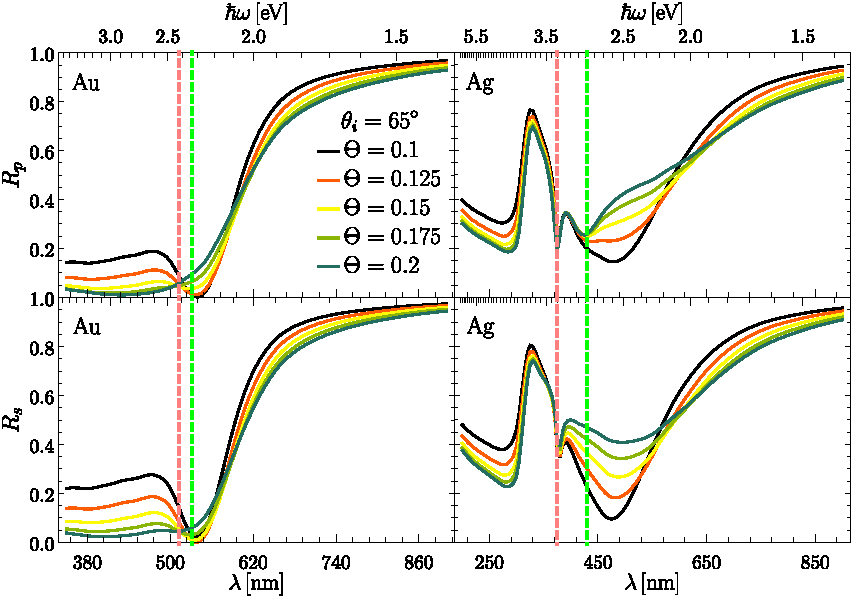
\includegraphics[scale=1]{2-Resultados/figs/6-AuThetaVar/0-cut65_Au_Aug.pdf}\vspace*{-.5em}
	\caption{Cortes a $\theta_i = 65^\circ$ de las gráficas de  la reflectancia  en configuración ATR  de una monocapa de NPs esféricas de oro de radio $a=25$ nm (Fig. \ref{fig:Au-R-Theta}) y de plata de $a=35$ nm (Fig. \ref{fig:Ag-R-Theta}) como función de la longitud de onda $\lambda$ (escala inferior) y de la energía $\hbar\omega$ (escala superior). Los paneles izquierdos corresponden a los cálculos para la monocapa de NPs de oro y los derechos a los de NPs de plata; los panles superiores corresponden a la reflectancia en polarización \emph{p} y los inferiores a polarización \emph{s}. La SP-SPR dipolar (líneas punteadas verticales verdes) para la NP de oro se localiza en  $\lambda \approx 531$ nm y la de la NP de plata en $\lambda\approx430$ nm, mientras la SP-SPR cuadrupolar (líneas punteadas verticales rosas) se localizan en $\lambda\approx513$ nm y en $\lambda\approx375$ nm para las NPs de oro y plata, respectivamente. }\label{fig:AuAg-Cuts-65}
	\end{figure}	
	
%Tanto para la monocapa de NPs de oro como de plata, la reflectancia a valores de $\lambda$ menores a los de la SP-SPR cuadrupolar es menor conforme la fracción de cubierta crece y este comportamiento se invierte para $\lambda$ mayores a la SP-SPR cuadrupolar.
En la Fig. \ref{fig:AuAg-Cuts-65} la reflectancia  para la monocapa de NPs de oro (paneles izquierdos) se observa la SP-SPR y el supuesto modo plasmónico colectivo para valores particulares de $\Theta$. Por ejemplo, a $\Theta=0.2$  (línea turquesa) a ambas polarizaciones no se observa la SP-SPR dipolar ($\lambda\approx531$ nm) ni tampoco el supuesto modo plasmónico colectivo,  pero  para $\Theta= 0.1$ (línea negra)  y $0.125$ (línea naranja), se observa que el supuesto modo colectivo se superpone con la SP-SPR dipolar. La longitud de onda de excitación $\lambda^{exc}$ del supuesto modo plasmónico colectivo para $\Theta=0.125$ es $\lambda^{exc} \approx 540\text {nm}$ y la reflectancia evaluada en $\lambda^{exc}$ es $R\approx 0$ para ambas polarizaciones,  mientras que  para $\Theta=0.1$,  $R_p(\lambda^{exc}) \approx 0$ y $R_s(\lambda^{exc})\approx 0.02$. %Para los valores intermedios de $\Theta$ la reflectancia a las longitudes de onda del supuesto modo plasmónico colectivo aumenta.

Para la monocapa de NPs de plata, paneles derechos en la Fig. \ref{fig:AuAg-Cuts-65}, la reflectancia a $\theta_i=65^\circ$, a todos los valores de $\Theta$, presenta un mínimo a $375$ nm (línea punteada vertical rosa) que corresponde a la SP-SPR cuadrupolar. La excitación dipolar de partícula individual a $430$ nm sólo es apreciable como mínimos locales en la reflectancia a polarización \emph{p}. Para polarización \emph{s} el supuesto modo plasmónico colectivo y la SP-SPR dipolar se traslapan. Los valores de la  reflectancia para la monocapa de NPs de plata considerando $\theta_i=65^\circ$ son mayores al aumentar $\Theta$ y siempre mayores a $0.2$, a diferencia de los resultados con NPs de oro en donde se obtuvieron valores cercanos a cero. Al igual que para el caso de NPs modeladas con un función dieléctrica tipo Drude, el supuesto modo plasmónico colectivo para una monocapa de NPs de oro y de plata se corre hacia el rojo conforme $\Theta$ crece.
	
	\begin{figure}[h!]\centering
	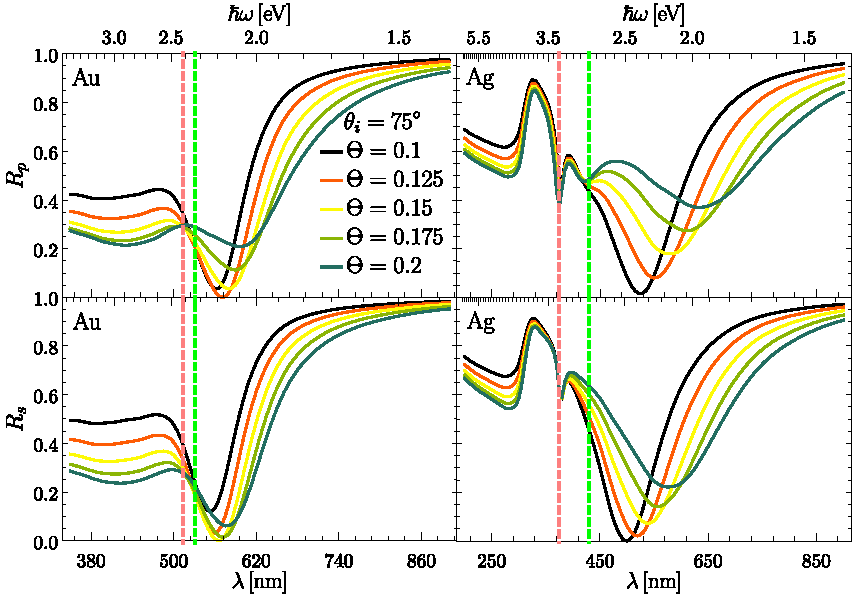
\includegraphics[scale=1]{2-Resultados/figs/6-AuThetaVar/0-cut75_Au_Aug.pdf}\vspace*{-.5em}
	\caption{Cortes a $\theta_i = 75^\circ$ de las gráficas de  la reflectancia  en configuración ATR  de una monocapa de NPs esféricas de oro de radio $a=25$ nm (Fig. \ref{fig:Au-R-Theta}) y de plata de $a=35$ nm (Fig. \ref{fig:Au-R-Theta}) como función de la longitud de onda $\lambda$ (escala inferior) y de la energía $\hbar\omega$ (escala superior). Los paneles izquierdos corresponden a los cálculos para la monocapa de NPs de oro y los derechos a los de NPs de plata; los panles superiores corresponden a la reflectancia en polarización \emph{p} y los inferiores a polarización \emph{s}. La SP-SPR dipolar (líneas punteadas verticales verdes) para la NP de oro se localiza en  $\lambda \approx 531$ nm y la de la NP de plata en $\lambda\approx430$ nm, mientras la SP-SPR cuadrupolar (líneas punteadas verticales rosas) se localizan en $\lambda\approx513$ nm y en $\lambda\approx370$ nm para las NPs de oro y plata, respectivamente.}\label{fig:AuAg-Cuts-75}
	\end{figure}	

%En contraste con los cortes a $\theta_i=65^\circ$ (Fig. \ref{fig:AuAg-Cuts-65}), en la reflectancia para $\theta_i=75^\circ$ (Fig. \ref{fig:AuAg-Cuts-75}) tanto para la monocapa de NPs de oro, como de plata, se aprecia el supuesto modo plasmónico colectivo a longitudes de onda mayores a la SP-SPR dipolar, además de haberse corrido al rojo respecto al caso de $\theta_i=65^\circ$ para todos los valores de $\Theta$ considerados. Para la monocapa de NPs de oro (paneles izquierdos en la Fig. \ref{fig:AuAg-Cuts-75}), la longitud de onda de excitación del supuesto modo plasmónico colectivo $\lambda^{exc}$ para $\Theta=0.1$ se localiza en $\lambda\approx570$ nm y en $\lambda\approx550$ nm para polarización \emph{p} y \emph{s}, respectivamente, mientras que para $\theta_i=75^\circ$ se localiza en $\lambda\approx 540$ nm para ambas polarizaciones. Sin embargo, el valor de la reflectancia en $\lambda^{exc}$ aumenta para ambas polarizaciones en comparación con la reflectancia a $\theta_i=65^\circ$. Por otro lado, para la monocapa de NPs de plata, para $\Theta=0.1$ en polarización \emph{p}, el supuesto modo plasmónico colectivo se corre a $\lambda^{exc}=490$ nm al evaluarse en $\theta_i=75^\circ$, mientras que para $\theta_i=65^\circ$ se localizaba en $470$ nm; para polarización \emph{s}, el supuesto modo plasmónico colectivo a $75^\circ$ se encuentra a $\lambda^{exc}=470$ nm y a $65^\circ$ a $455$ nm; adicionalmente $R(\lambda^{exc})\approx 0$ para $\theta_i=75^\circ$, es decir, que es menor en comparación al caso de $\theta_i=65^\circ$. El corrimiento al rojo de $\lambda^{exc}$ es un comportamiento observado para todos los valores de $\Theta$ para ambas monocapas (oro y plata).

En contraste con los cortes a $\theta_i=65^\circ$ (Fig. \ref{fig:AuAg-Cuts-65}), la reflectancia para $\theta_i=75^\circ$ (Fig. \ref{fig:AuAg-Cuts-75}) tanto para la monocapa de NPs de oro, como de plata, se aprecia el supuesto modo plasmónico colectivo a longitudes de onda mayores a la SP-SPR dipolar, además de haberse corrido al rojo respecto al caso de $\theta_i=65^\circ$ para todos los valores de $\Theta$ considerados. Una característica compartida por todos los casos estudiados de $\Theta$, al comparar los cortes para $\theta_i=65^\circ$ (Fig. \ref{fig:AuAg-Cuts-65}) y para $\theta_i=75^\circ$ (Fig. \ref{fig:AuAg-Cuts-75}), es una mejor definición en la forma de la resonancia y de su FWHM. Por ejemplo, para la monocapa de NPs de plata, para los dos ángulos de incidencia elegidos y el caso de $\Theta=0.2$ considerando polarización \emph{s} (líneas turquesas en los paneles inferiores izquierdos), la resonancia es menos amplia y mejor definida para $\theta_i=75^\circ$ ($\Gamma=160$ nm) que para $\theta_i=65^\circ$ ($\Gamma=220$ nm).% Lo análogo sucede para la monocapa de NPs de oro al considerar fracciones de cubierta mayores a $0.175$.% En contraste, los valores de la reflectancia a $\lambda^{exc}$ para la monocapa de NPs de oro y de plata no son similares: para las NPs de oro, $R_p\approx 0$ cuando $\Theta=0.125$ (línea naranja) y $R_s\approx 0$ para $\Theta=0.15$ (línea amarilla) mas para las NPs de plata $R\approx 0$, para ambas polarizaciones, cuando $\Theta=0.1$ (línea negra). Es decir, para los valores de fracciones de cubierta $\Theta$ elegidos, considerando NPs de oro de de $25$ nm y de plata de $35$ nm, la optimización de la monocapa para el biosensado es distinta.

Para determinar si los radios elegidos para las NPs de oro y de plata son los óptimos para el empleo del supuesto modo plasmónico colectivo en el sensado (valores de $R\approx 0$ dentro del espectro visible y considerando $\theta_i<80^\circ$), se presentan a continuación gráficas de la reflectancia en configuración ATR para una monocapa de NPs de oro (Fig. \ref{fig:Au-R-Rad}) y de plata (Fig. \ref{fig:Ag-R-Rad}) para un valor de fracción de cubierta $\Theta$ fijo y para distintos radios $a$ de las NPs. En la Fig. \ref{fig:Au-R-Rad} se grafica la reflectancia en configuración ATR para una monocapa de NPs de oro, inmersa en un medio con $n_m=1.33$ y soportada por un sustrato con $n_s=1.5$, considerando  $\Theta=0.125$, fracción de cubierta elegida con base en los resultados calculados en las Figs. \ref{fig:AuAg-Cuts-65} y \ref{fig:AuAg-Cuts-75}, variando los radios de las NPs alrededor de $25$ nm, es decir, $a=15$ nm, $20$ nm, $25$ nm, $30$ nm y $35$ nm, siendo entonces las SP-SPR dipolares (líneas punteadas verticales verdes) $\lambda\approx 525$ nm, $527$ nm, $531$ nm, $535$ nm y $541$ nm para cada radio, respectivamente, y las cuadrupolares (líneas punteadas verticales rosas) $\lambda\approx 513$ nm para $a=15$ nm, $20$ nm y $25$ nm, y $\lambda\approx 514$ nm para $a=30$ nm y $35$ nm; el supuesto modo plasmónico colectivo se representa mediante los punto amarillos.

\begin{figure}[t!]\centering
\hspace*{-.5em}\begin{tikzpicture}[scale=1]
\node[inner sep=0pt] (graf) at (-.15,0){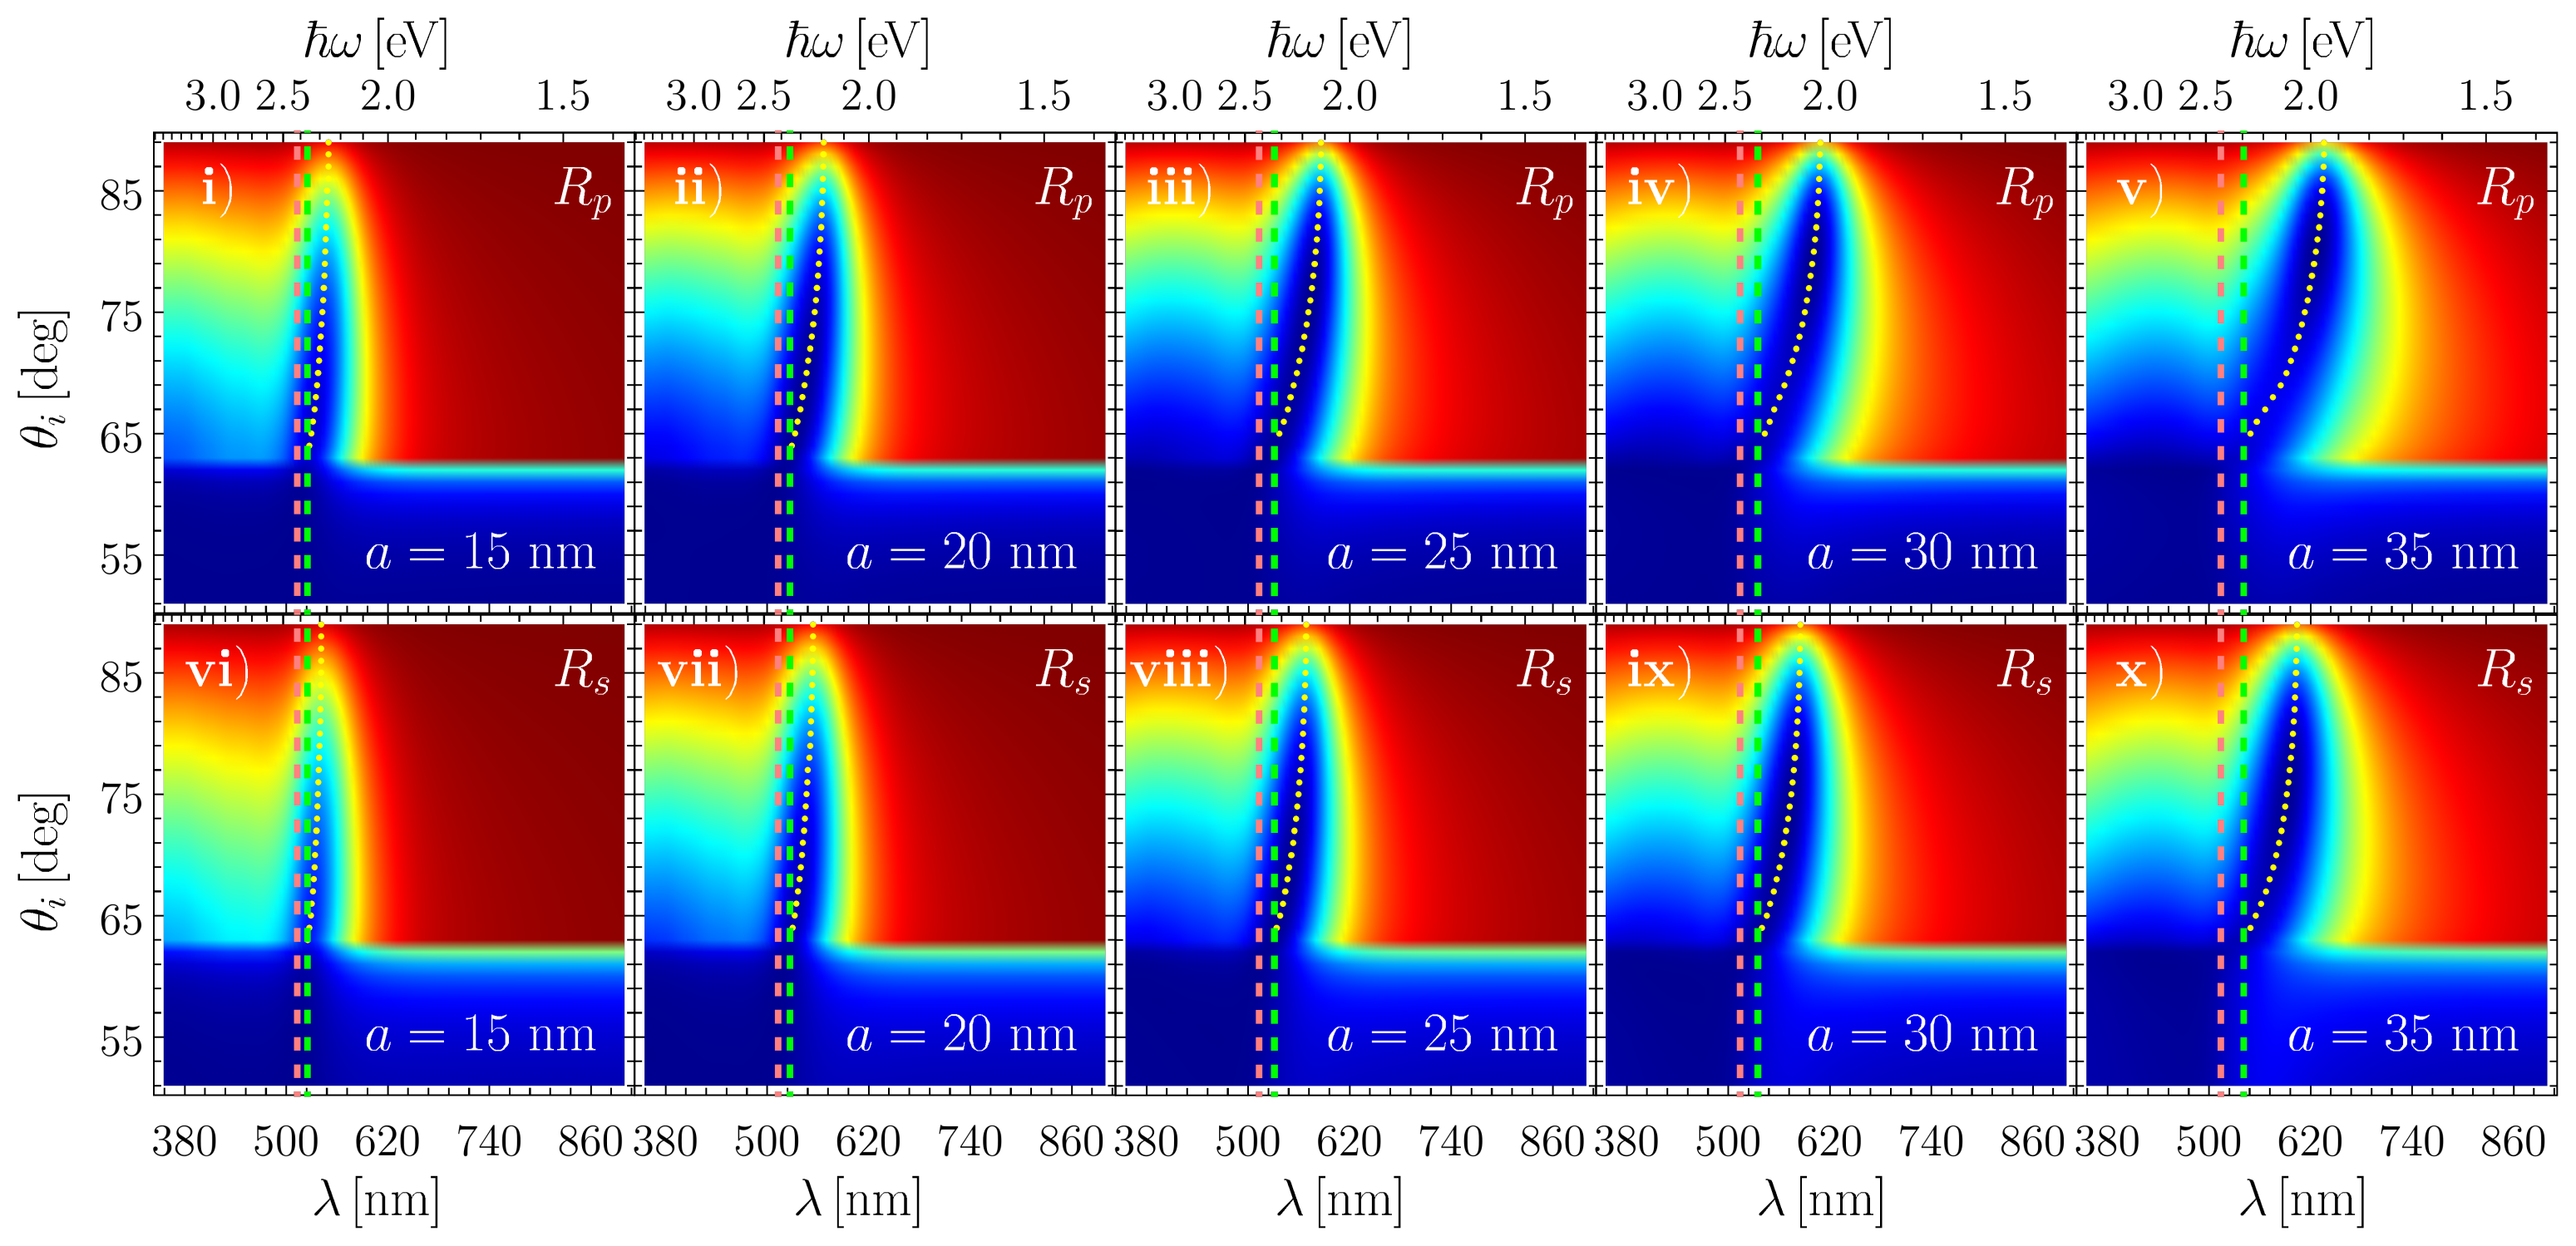
\includegraphics[scale=1]{2-Resultados/figs/8-AurVar/0-2D_Grid}};
\node[right, inner sep=0pt] (legend) at (7.1,.15) {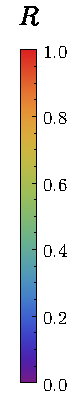
\includegraphics[scale=1, trim={00 -15 00 00}, clip]{2-Resultados/figs/0-RBar_v}};

\def\y{4.2}
	\node at(-5.2,\y){\normalsize $a = 15 $ nm};
	\node at(-2.4,\y){\normalsize $a = 20 $ nm};
	\node at(0.4,\y) {\normalsize $a = 25$ nm};
	\node at(3.2,\y) {\normalsize $a = 30 $ nm};
	\node at(6.0,\y) {\normalsize $a = 35 $ nm};

\def\xR{7}
\def\yR{2.5}	
	\node at(\xR,\yR){$R_p $};
	\node at(\xR,\yR-2.8){$R_s$};
\end{tikzpicture}\vspace*{-.5em}
	\caption{Gráficas de la reflectancia de una monocapa de NPs de oro en configuración ATR como función del ángulo de incidencia $\theta_i$ y de la longitud de onda $\lambda$ (escala inferior), así como de la energía  $\hbar\omega$ (escala superior).  Las gráficas   en el renglón superior [\textbf{i)--v)}] muestran los resultados para  polarización \emph{p} y las del renglón inferior  [\textbf{vi)}--\textbf{x)}]  para polarización  \emph{s}, donde se consideró una fracción de cubierta $\Theta = 0.125$ y  NPs de radio  $a$: $15$ nm, $20$ nm, $25$ nm, $30$ nm y $35$ nm.  Las líneas verticales punteadas verdes y rosas corresponden a las SP-SPRs dipolar y  cuadrupolar, respectivamente.  Los puntos amarillos corresponden a los mínimos en $R$ para ángulos mayores a $\theta_c\approx 62.5^\circ$ y longitudes de onda mayores a la SP-SPRs dipolar.}	\label{fig:Au-R-Rad}	
	\end{figure}	

En la Fig. \ref{fig:Au-R-Rad} se observa la tendencia identificada con la monocapa de NPs con una función dieléctrica tipo Drude al variar el tamaño de las NPs: a radios mayores, el supuesto modo plasmónico colectivo se corre al rojo y el ancho de la resonancia aumenta; conforme el radio disminuye, el supuesto modo plasmónico colectivo tiende a la frecuencia de la SP-SPR dipolar. Al igual que la respuesta EM de la monocapa de NPs de oro ante variaciones de la fracción de cubierta (Fig. \ref{fig:Au-R-Theta}),  el supuesto modo plasmónico colectivo a la longitud de onda de la SP-SPR dipolar se excita a partir de un ángulo de incidencia, aumentando conforme $\Theta$ crece.% Por otro lado, al considerar el parámetro $\Theta$ fijo y variar el radio de las NPs (Fig. \ref{fig:Au-R-Rad}), el supuesto modo plasmónico colectivo se excita, a la longitud de onda de la SP-RPR dipolar,  a partir del mismo ángulo de incidencia ($\theta_i\approx 65^\circ$) para todos los valores de $a$ considerados.

En la Fig. \ref{fig:Ag-R-Rad}	 se presentan los cálculos de la reflectancia de una monocapa de NPs  de plata, inmersa en un medio con $n_m=1.33$ y soportada por un sustrato con $n_s=1.5$ en configuración ATR. Se considera  $\Theta=0.1$ por ser la fracción de cubierta a la cual $R\approx 0$ en las Figs. \ref{fig:AuAg-Cuts-65} y \ref{fig:AuAg-Cuts-75}, y los radios de las NPs alrededor de $35$ nm, es decir, $a=30$ nm, $35$ nm, $40$ nm, $45$ nm y $50$ nm, estando entonces las SP-SPR dipolares (líneas punteadas verticales verdes) localizadas en $\lambda\approx 417$ nm, $430$ nm, $444$ nm, $459$ nm y $479$ nm para cada radio, respectivamente, y las cuadrupolares (líneas punteadas verticales rosas) en $\lambda\approx 373$ nm, $376$ nm, $379$ nm, $383$ nm y $388$ nm, respectivamente. Los puntos amarillos corresponden al mínimos de la reflectancia del supuesto modo plasmónico colectivo, cuyo comportamiento es semejante al observado para el oro en la Fig. \ref{fig:Au-R-Rad}: al aumentar el radio de las NPs, el supuesto modo plasmónico colectivo es más apreciable y se corre hacia el rojo, efecto más evidente para polarización \emph{p} que para \emph{s}, mientras que el ensanchamiento del supuesto modo plasmónico colectivo es mayor para las NPs de plata debido a que el radio de las NPs es mayor que el de las NPs de oro. A pesar de esta similitud en el comportamiento del supuesto modo plasmónico colectivo para NPs de oro y de plata, una diferencia son los valores de $\theta_i$ a los cuales la reflectancia se minimiza: el mínimo global de la reflectancia debido al supuesto modo plasmónico colectivo se localiza a ángulos rasantes conforme aumenta el radio de las NPs oro, mientras que para las NPs de plata, el mínimo global se corre a ángulos cercanos al ángulo crítico.

Para contrastar el comportamiento del supuesto modo plasmónico ante variaciones de $\Theta$ contra variaciones en $a$,  se grafican en la Fig. \ref{fig:AuAg-Cuts-Rad-65} cortes a $\theta_i = 65^\circ$  y en la  Fig.  \ref{fig:AuAg-Cuts-Rad-75} a $75^\circ$ de la reflectancia $R$ de las Figs. \ref{fig:Au-R-Rad} y \ref{fig:Ag-R-Rad}, con la finalidad de observar a qué longitud de onda se sintoniza el supuesto modo plasmónico colectivo a los valores de $\theta_i$ seleccionados, así como el ancho de su resonancia, y elegir los parámetros óptimos para su uso en el sensado. Tanto en la Fig. \ref{fig:AuAg-Cuts-Rad-65}, como en la Fig. \ref{fig:AuAg-Cuts-Rad-75}, los paneles izquierdos corresponden a los cálculos para una monocapa de NPs de oro con $\Theta=0.125$ y los derechos para una monocapa de NPs de plata con $\Theta=0.1$, mientras que los paneles superiores corresponden a polarización \emph{p} y los inferiores a \emph{s}.

\begin{figure}[h!]\centering
\hspace*{-.5em}\begin{tikzpicture}[scale=1]
\node[inner sep=0pt] (graf) at (-.15,0){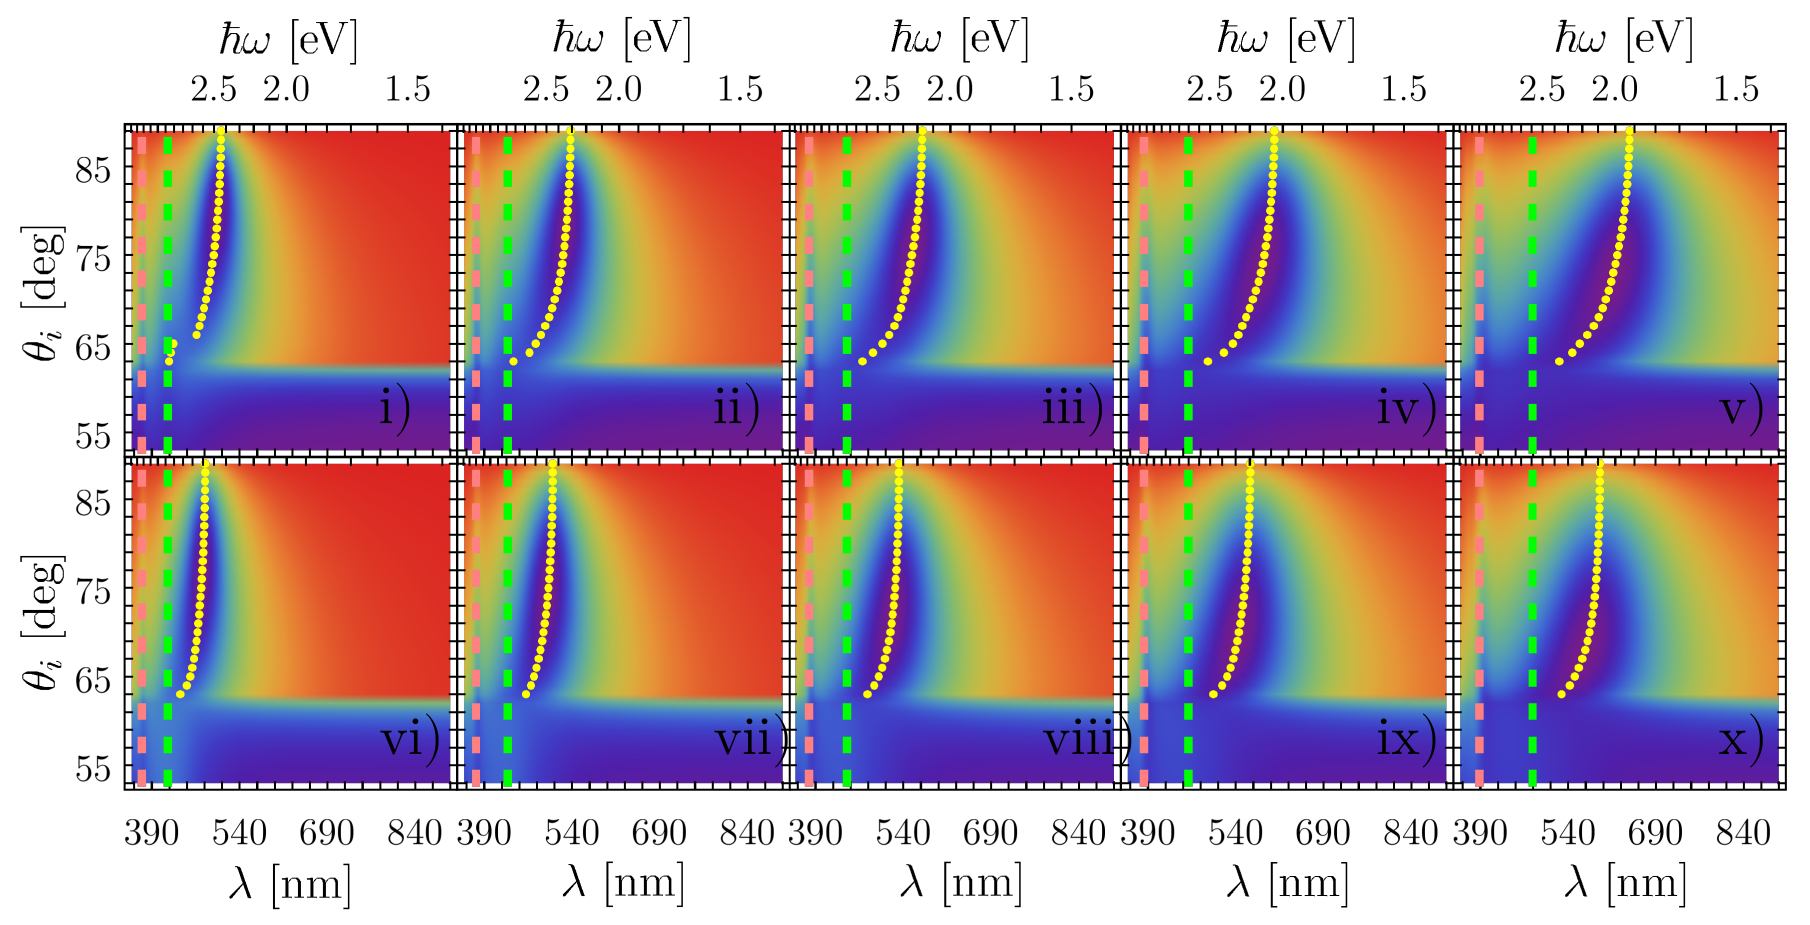
\includegraphics[scale=1]{2-Resultados/figs/9-AgrVar/0-2D_Grid}};
\node[right, inner sep=0pt] (legend) at (7.1,.15) {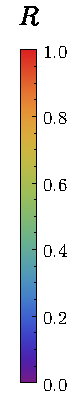
\includegraphics[scale=1, trim={00 -15 00 00}, clip]{2-Resultados/figs/0-RBar_v}};

\def\y{4.2}
	\node at(-5.2,\y){\normalsize $a = 30 $ nm};
	\node at(-2.4,\y){\normalsize $a = 35 $ nm};
	\node at(0.4,\y) {\normalsize $a = 40 $nm};
	\node at(3.2,\y) {\normalsize $a = 45 $ nm};
	\node at(6.0,\y) {\normalsize $a = 50 $ nm};

\def\xR{7}
\def\yR{2.5}	
	\node at(\xR,\yR){$R_p $};
	\node at(\xR,\yR-2.8){$R_s$};
\end{tikzpicture}\vspace*{-.5em}
	\caption{Gráficas de la reflectancia de una monocapa de NPs de plata en configuración ATR como función del ángulo de incidencia $\theta_i$ y de la longitud de onda $\lambda$ (escala inferior), así como de la energía  $\hbar\omega$ (escala superior).  Las gráficas   en el renglón superior [\textbf{i)--v)}] muestran los resultados para  polarización \emph{p} y las del renglón inferior  [\textbf{vi)}--\textbf{x)}]  para polarización  \emph{s}, donde se consideró una fracción de cubierta $\Theta = 0.1$ y  NPs de radio  $a$: $30$ nm, $35$ nm, $40$ nm, $45$ nm y $50$ nm.  Las líneas verticales punteadas verdes y rosas corresponden a las SP-SPRs dipolar y  cuadrupolar, respectivamente.  Los puntos amarillos corresponden a los mínimos en $R$ para ángulos mayores a $\theta_c\approx 62.5^\circ$ y longitudes de onda mayores a la SP-SPRs dipolar.
}	\label{fig:Ag-R-Rad}	
	\end{figure}	

Los cálculos de la reflectancia de la monocapa de NPs de oro a $\theta_i=65^\circ$, considerando ambas polarizaciones (paneles izquierdos de la Fig. \ref{fig:AuAg-Cuts-Rad-65}), muestran que el ancho de la excitación del supuesto modo plasmónico colectivo disminuye  al disminuir el radio de las NPs, por ejemplo a para $a=15$ nm (línea negra) la FWHM para \emph{p} es $\Gamma=100$ nm y para \emph{s} es $\Gamma=110$ nm, mientras que para $25$ nm (línea amarilla), el ancho de la resonancia es $\Gamma=110$ nm y $\Gamma=125$  nm, para \emph{p} y \emph{s}, respectivamente. La presencia del supuesto modo plasmónico colectivo es menos evidente para los radios mayores, como se observa para $a=35$ nm (línea turquesa), donde éste se excita a $\lambda^{exc}\approx 550$ nm para ambas polarizaciones. Por otro lado, para ambas polarizaciones, la reflectancia de la monocapa de NPs de oro con $a=35$ nm en el intervalo  $\lambda<\lambda^{exc}$  es menor a $0.1$ por lo que el supuesto modo plasmónico colectivo no es tan apreciable como para el caso de $a=20$ nm (línea naranja) en donde $R\approx 0$ en $\lambda^{exc}\approx 530$. Es decir, para ángulos cercanos al ángulo crítico, las NPs de oro de menor tamaño son más aptas para el biosensado, así como valores de $\Theta$ cercanos a $0.125$.

	\begin{figure}[h!]\centering
	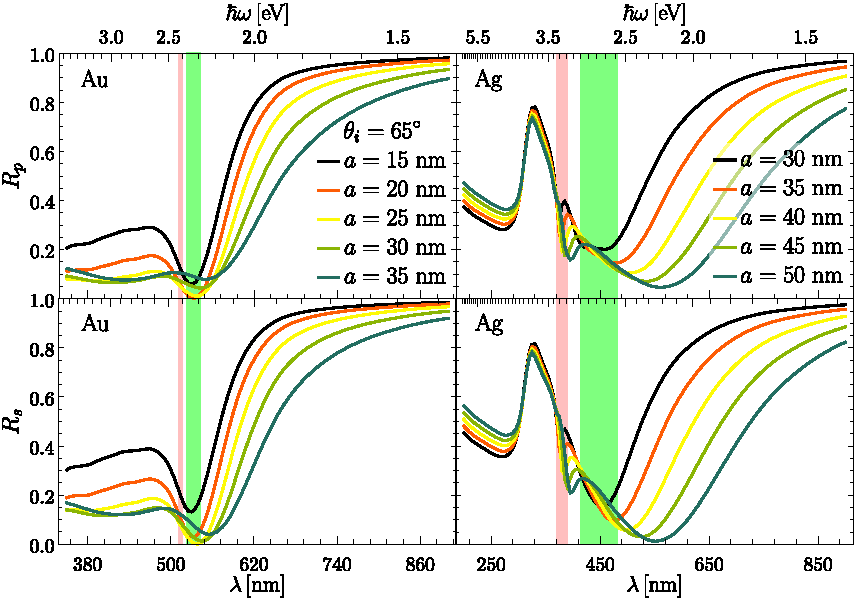
\includegraphics[scale=1]{2-Resultados/figs/8-AurVar/0-cut65_Au_Aug.pdf}\vspace*{-.5em}
	\caption{Cortes a $\theta_i = 65^\circ$ de las gráficas de  la reflectancia  en configuración ATR  de una monocapa de NPs esféricas de oro con $\Theta=0.125$ (Fig. \ref{fig:Au-R-Rad}) y de plata con $\Theta=0.1$ (Fig. \ref{fig:Ag-R-Rad}) como función de la longitud de onda $\lambda$ (escala inferior) y de la energía $\hbar\omega$ (escala superior). Los paneles izquierdos corresponden a los cálculos para la monocapa de NPs de oro y los derechos a los de NPs de plata; los panles superiores corresponden a la reflectancia en polarización \emph{p} y los inferiores a polarización \emph{s}. Los valores de radios $a$ considerados para la monocapa de NPs de oro fueron  $a=15$ nm, $20$ nm, $25$ nm, $30$ nm y $35$ nm, localizando las SP-SPR dipolares (región sombreada verde) entre $525\mbox{ nm}<\lambda<541\mbox{ nm}$ y las cuadrupolares  (región sombreada verde) entre $513$ nm y $514$ nm; para la monocapa de NPs de plata se escogieron los radios  $a=30$ nm, $35$ nm, $40$ nm, $45$ nm y $50$ nm, por lo que las SP-SPR dipolares se encuentran entre $417\mbox{ nm}<\lambda<479\mbox{ nm}$ y las cuadrupolares $373\mbox{ nm}<\lambda<388\mbox{ nm}$.}\label{fig:AuAg-Cuts-Rad-65}
	\end{figure}

Al observar la reflectancia de la monocapa de NPs de plata a $65^\circ$ (paneles derechos en la Fig. \ref{fig:AuAg-Cuts-Rad-65}), el efecto del ensanchamiento del supuesto modo plasmónico colectivo, así como el corrimiento al rojo es más evidente comparado al caso de NPs de oro (paneles izquierdos). Esto se debe a  que los valores considerados para los radios de las NPs fueron mayores que para el oro. Para polarización \emph{s} (panel inferior derecho), el ancho del supuesto modo plasmónico colectivo para un radio de $a=30$ nm (línea negra) se localiza en $\lambda^{exc}\approx 450$ nm y tiene un FWHM $\Gamma$ de $160$ nm, mientras que para un radio de $50$ nm (línea turquesa), el supuesto modo plasmónico colectivo se excita a $\lambda^{exc}\approx 550$ nm y $\Gamma\approx 250$ nm, es decir, $1.5$ veces mayor en comparación al caso con $a=30$ nm. Para polarización \emph{p}, considerando NPs de plata, la detección del supuesto modo plasmónico colectivo se complica en comparación al caso de polarización \emph{s} dado que los valores de $\Gamma$ son, para todos los valores de $a$ considerados, al menos $40$ nm menores para \emph{s} que para \emph{p}. Asimismo, para polarización \emph{p} la resonancia a $\lambda^{exc}$ muestra un comportamiento cualitativo distinto para $\lambda\lessapprox\lambda^{exc}$ que $\lambda\gtrapprox\lambda^{exc}$, a diferencia de los resultados para \emph{s}, donde el supuesto modo plasmónico colectivo presenta un comportamiento más simétrico alrededor de $\lambda^{exc}$. A pesar de la distinta forma de la resonancia según la polarización, las resonancias a ambas polarizaciones pueden identificarse ya que la SP-SPR cuadrupolar no se traslapa con el supuesto modo plasmónico colectivo y se aprecia como un mínimo en la reflectancia. Las NPs de plata de mayor tamaño y fracciones de cubierta bajas ($\Theta= 0.1$) permiten el empleo de la monocapa para el sensado al elegir ángulos cercanos a $\theta_c$, pues el supuesto modo plasmónico colectivo se sintoniza en el espectro visible, además de alcanzar valores de $R$ cercanos a cero y tener formas más definidas, en comparación a valores mayores de $\Theta$ (ver Fig. \ref{fig:AuAg-Cuts-65}), sobre todo en polarización \emph{s}.

Cuando se varió el parámetro $\Theta$ manteniendo el radio de las NPs de oro y de plata fijo (Figs. \ref{fig:AuAg-Cuts-65} y \ref{fig:AuAg-Cuts-75}), se observó que para $\theta_i=75^\circ$  el supuesto modo plasmónico colectivo tenía una mejor definición en comparación a $\theta_i =65^\circ$, además de sintonizarse más hacia al rojo y, para los valores de $\Theta$ seleccionados, la reflectancia disminuía. Estas características también se observan en la variación del radio de las NPs en la monocapa, comparando $\theta_i=65^\circ$ (Fig. \ref{fig:AuAg-Cuts-Rad-65}) y $\theta_i=75^\circ$ (Fig. \ref{fig:AuAg-Cuts-Rad-75})  con un valor de $\Theta=0.125$ para las NPs de oro (paneles izquierdos) y de $\Theta=0.1$ para las de plata (paneles derechos). Al considerar NPs de oro, la reflectancia a $\theta_i= 65^\circ$ (Fig. \ref{fig:AuAg-Cuts-Rad-65})  toma valores alrededor de $0.5$ para $350$ nm $\leq \lambda\leq 525$ nm lo que contrasta con los valores a las longitudes de onda del supuesto modo plasmónico colectivo $\lambda^{exc}$ en donde, para polarización \emph{p}, $R_p(\lambda^{exc})<0.025$ para radios de $a\geq 20$ nm (líneas naranja, amarilla, verde y turquesa) y, para \emph{s} $R_s(\lambda^{exc})<0.025$ cuando $a\geq 25$ nm (líneas amarilla, verde y turquesa). Adicionalmente, para los radios  $a\geq 25$ nm, que cumplen para ambas polarizaciones que $R(\lambda^{exc})<0.025$, el supuesto modo plasmónico colectivo se sintoniza en el intervalo entre $\lambda\approx 520$ nm y $\lambda\approx 620$ nm, y el ancho de la resonancia es de $\Gamma \approx 100$ nm para $a=25$ nm y de $\Gamma\approx 130$ nm para $a=35$ nm. Al tener una respuesta EM semejante para radios entre $25$ nm y $35$ nm, el supuesto modo plasmónico colectivo presente en una monocapa de NPs de oro, a ambas polarizaciones y considerando $\theta_i=75^\circ$, puede emplearse para sensado, ya que errores experimentales en la fabricación de las NPs no modificarían en una forma significativa la respuesta promedio.


	\begin{figure}[h!]\centering
	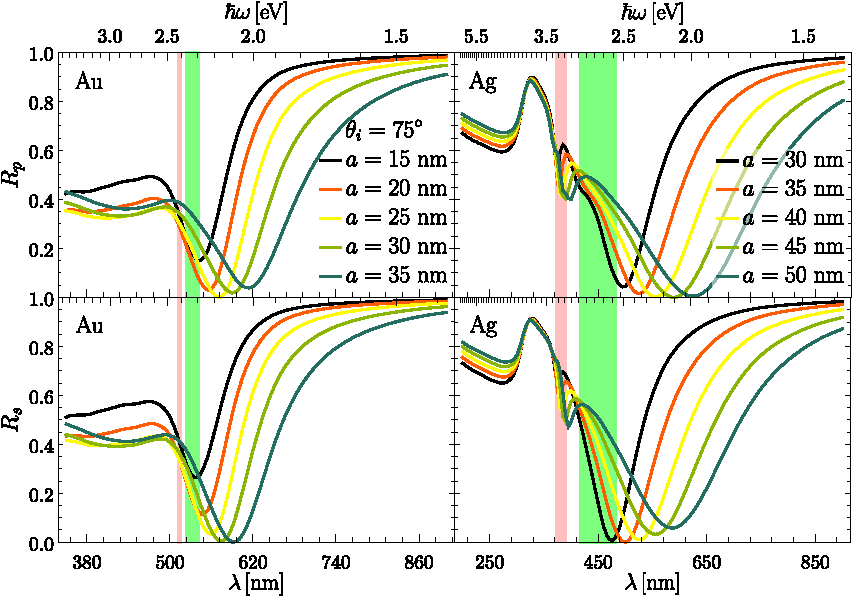
\includegraphics[scale=1]{2-Resultados/figs/8-AurVar/0-cut75_Au_Aug.pdf}\vspace*{-.5em}
	\caption{Cortes a $\theta_i = 75^\circ$ de las gráficas de  la reflectancia  en configuración ATR  de una monocapa de NPs esféricas de oro con $\Theta=0.125$ (Fig. \ref{fig:Au-R-Rad}) y de plata con $\Theta=0.1$ (Fig. \ref{fig:Ag-R-Rad}) como función de la longitud de onda $\lambda$ (escala inferior) y de la energía $\hbar\omega$ (escala superior). Los paneles izquierdos corresponden a los cálculos para la monocapa de NPs de oro y los derechos a los de NPs de plata; los panles superiores corresponden a la reflectancia en polarización \emph{p} y los inferiores a polarización \emph{s}. Los valores de radios $a$ considerados para la monocapa de NPs de oro fueron  $a=15$ nm, $20$ nm, $25$ nm, $30$ nm y $35$ nm, localizando las SP-SPR dipolares (región sombreada verde) entre $525\mbox{ nm}<\lambda<541\mbox{ nm}$ y las cuadrupolares  (región sombreada rosa) entre $513$ nm y $514$ nm; para la monocapa de NPs de plata se escogieron los radios  $a=30$ nm, $35$ nm, $40$ nm, $45$ nm y $50$ nm, por lo que las SP-SPR dipolares se encuentran entre $417\mbox{ nm}<\lambda<479\mbox{ nm}$ y las cuadrupolares entre $373\mbox{ nm}<\lambda<388\mbox{ nm}$.}\label{fig:AuAg-Cuts-Rad-75}
	\end{figure}	

Para la monocapa de NPs de plata (paneles derechos de la Fig. \ref{fig:AuAg-Cuts-Rad-75}), el comportamiento es análogo al observado para la monocapa de NPs de oro. La refelctancia evaluada en las longitudes de onda del supuesto modo plasmónico colectivo $\lambda^{exc}$, para la monocapa de las NPs de plata a ambas polarizaciones, es cercana a cero mientras que a longitudes de onda menores a la SP-SPR cuadrupolar, la cual puede observase como mínimos locales en $R$ alrededor de la región sombreada rosa, es mayor a $0.6$, por lo que se facilitaría experimentalmente la identificación del supuesto modo plasmónico colectivo. Por ejemplo, para polarización \emph{p} (panel superior derecho) para $a=40$ nm, $45$ nm y $50$ nm, el supuesto modo plasmónico colectivo se localiza a $500$ nm, $530$ nm y $540$ nm, respectivamente, y para estos tres casos $R_p\approx 0$. Asimismo, para polarización \emph{s} (panel inferior derecho) para $a=30$ nm, $35$ nm y $40$ nm, el supuesto modo plasmónico colectivo se excita a $\lambda^{exc}=460$ nm, $470$ nm y $480$ nm, respectivamente, e igualmente, $R_s\approx 0$. En general, para todos los casos de radios de NPs de plata mostrados en la Fig. \ref{fig:AuAg-Cuts-Rad-75}, la reflectancia a las longitudes de ondas del supuesto modo plasmónico colectivo es menor a $0.04$ a ambas polarizaciones. Los valores de la FWHM $\Gamma$ del supuesto modo plasmónico colectivo presente en la monocapa de NPs de plata y para los casos donde $R_s\approx R_p \approx 0$, son, para polarización \emph{p} de $\Gamma=80$ nm para $a=40$ nm (línea amarilla en el panel superior derecho) y $\Gamma=140$ nm para $a=50$ nm (línea turquesa en el panel superior derecho), mientras que para polarización \emph{s}, $\Gamma$ está en un rango entre $60$ nm, para $a=30$ nm (línea negra en el panel inferior derecho), y $80$ nm, para $a=40$ nm (línea amarilla en el panel inferior derecho). Al igual que con la monocapa de NPs de oro, empleando NPs de plata, el supuesto modo plasmónico colectivo puede emplearse en el sensado al considerar $\Theta=0.1$ y radios de NPs entre $35$ nm y $40$ nm, pues a $\theta_i=75^\circ$, la reflectancia (para ambas polarizaciones) a las longitudes de onda  $\lambda^{exc}$ que excitan al supuesto modo plasmónico colectivo es cercana a cero y representa un mínimo en la reflectancia global.


Con base en los resultados mostrados en las Figs. \ref{fig:AuAg-Cuts-75} y \ref{fig:AuAg-Cuts-Rad-75}, se propone que, para emplear una monocapa desordenada de NPs esféricas como sensor basado en el supuesto modo plasmónico colectivo, se eligen los parámetros $\Theta=0.125$ y radio $a=30$ nm con NPs de oro, y $\Theta=0.1$ y $a=40$ nm con NPs de plata. Estos parámetros garantizan la validez del CSM \cite{garcia2012multiple}. Finalmente, para determinar si el supuesto modo plasmónico colectivo en materiales reales tiene propiedades de un modo guiado, como las LSPR reportadas en \cite{kabashin2009plasmonic} o como se observó con el CSM al considerar una monocapa de NPs cuya función dieléctrica se describió por el modelo de Drude-Sommerfeld, se  muestran en la Fig. \ref{fig:RT-AuAg}  los cálculos de la reflectancia $R$, la transmitancia $T$ y la suma de éstas ($R+T$) de una monocapa de NPs inmersa en un medio con índice de refracción $n_m=1.33$ y soportada por un sustrato con índice de refracción $n_s=1.5$, en función del ángulo de incidencia $\theta_i$, así como de la longitud de onda $\lambda$ (escala inferior) y de la energía  $\hbar\omega$ (escala superior) de la onda plana incidente, tanto para polarización \emph{p}  [\textbf{i)}--\textbf{iii)}] como para \emph{s} [\textbf{iv)}--\textbf{vi)}]. La Fig. \ref{sfig:RT-Au} corresponde a los cálculos al considerar una monocapa de NPs de oro de radio de $30$ nm y con $\Theta=0.125$, y la  Fig. \ref{sfig:RT-Ag} a los de una monocapa de NPs de plata con radios de $40$ nm y $\Theta=0.1$, es decir, los óptimos para emplear el supuesto modo plasmónico colectivo en el sensado considerando $\theta_i<80^\circ$.

Los resultados de $R+T$, tanto para la monocapa de NPs de oro [paneles \textbf{iii)} y \textbf{vi)} en la Fig. \ref{sfig:RT-Au}] como para las de plata [paneles \textbf{iii)} y \textbf{vi)} en la Fig. \ref{sfig:RT-Ag}], muestran un comportamiento análogo al observado en el caso donde se emplearon las funciones dieléctricas tipo Drude para las NPs de la monocapa: la reflectancia a las longitudes de onda del supuesto modo plasmónico colectivo (puntos amarillos) es cercana a cero, además de que la transmitancia a esas mismas longitudes de onda es cero. En analogía con el SPP, en donde $R\approx T\approx 0$ a sus longitudes de onda de excitación, se refuerza la idea de que el supuesto modo plasmónico colectivo presenta las propiedades de un modo guiado cuando se consideran materiales reales para las NPs. A pesar de que a las longitudes de onda del supuesto modo plasmónico colectivo puede presentarse absorción, una parte de la energía que no viaja en las direcciones coherentes de reflexión o transmisión, puede propagarse a lo largo de la interfaz, por medio de procesos de esparcimiento múltiple por la interacción entre las NPs de la monocapa.

\begin{figure}[t!]\centering\noindent\hspace*{-5em}
	\begin{subfigure}{.01\linewidth}\caption{}\label{sfig:RT-Au}\vspace{5.5cm}\end{subfigure}
	\begin{subfigure}{.7\linewidth}\hspace*{-.5em}
	\begin{tikzpicture}[scale=1]
\node[inner sep=0pt] (graf) at (0.05,0){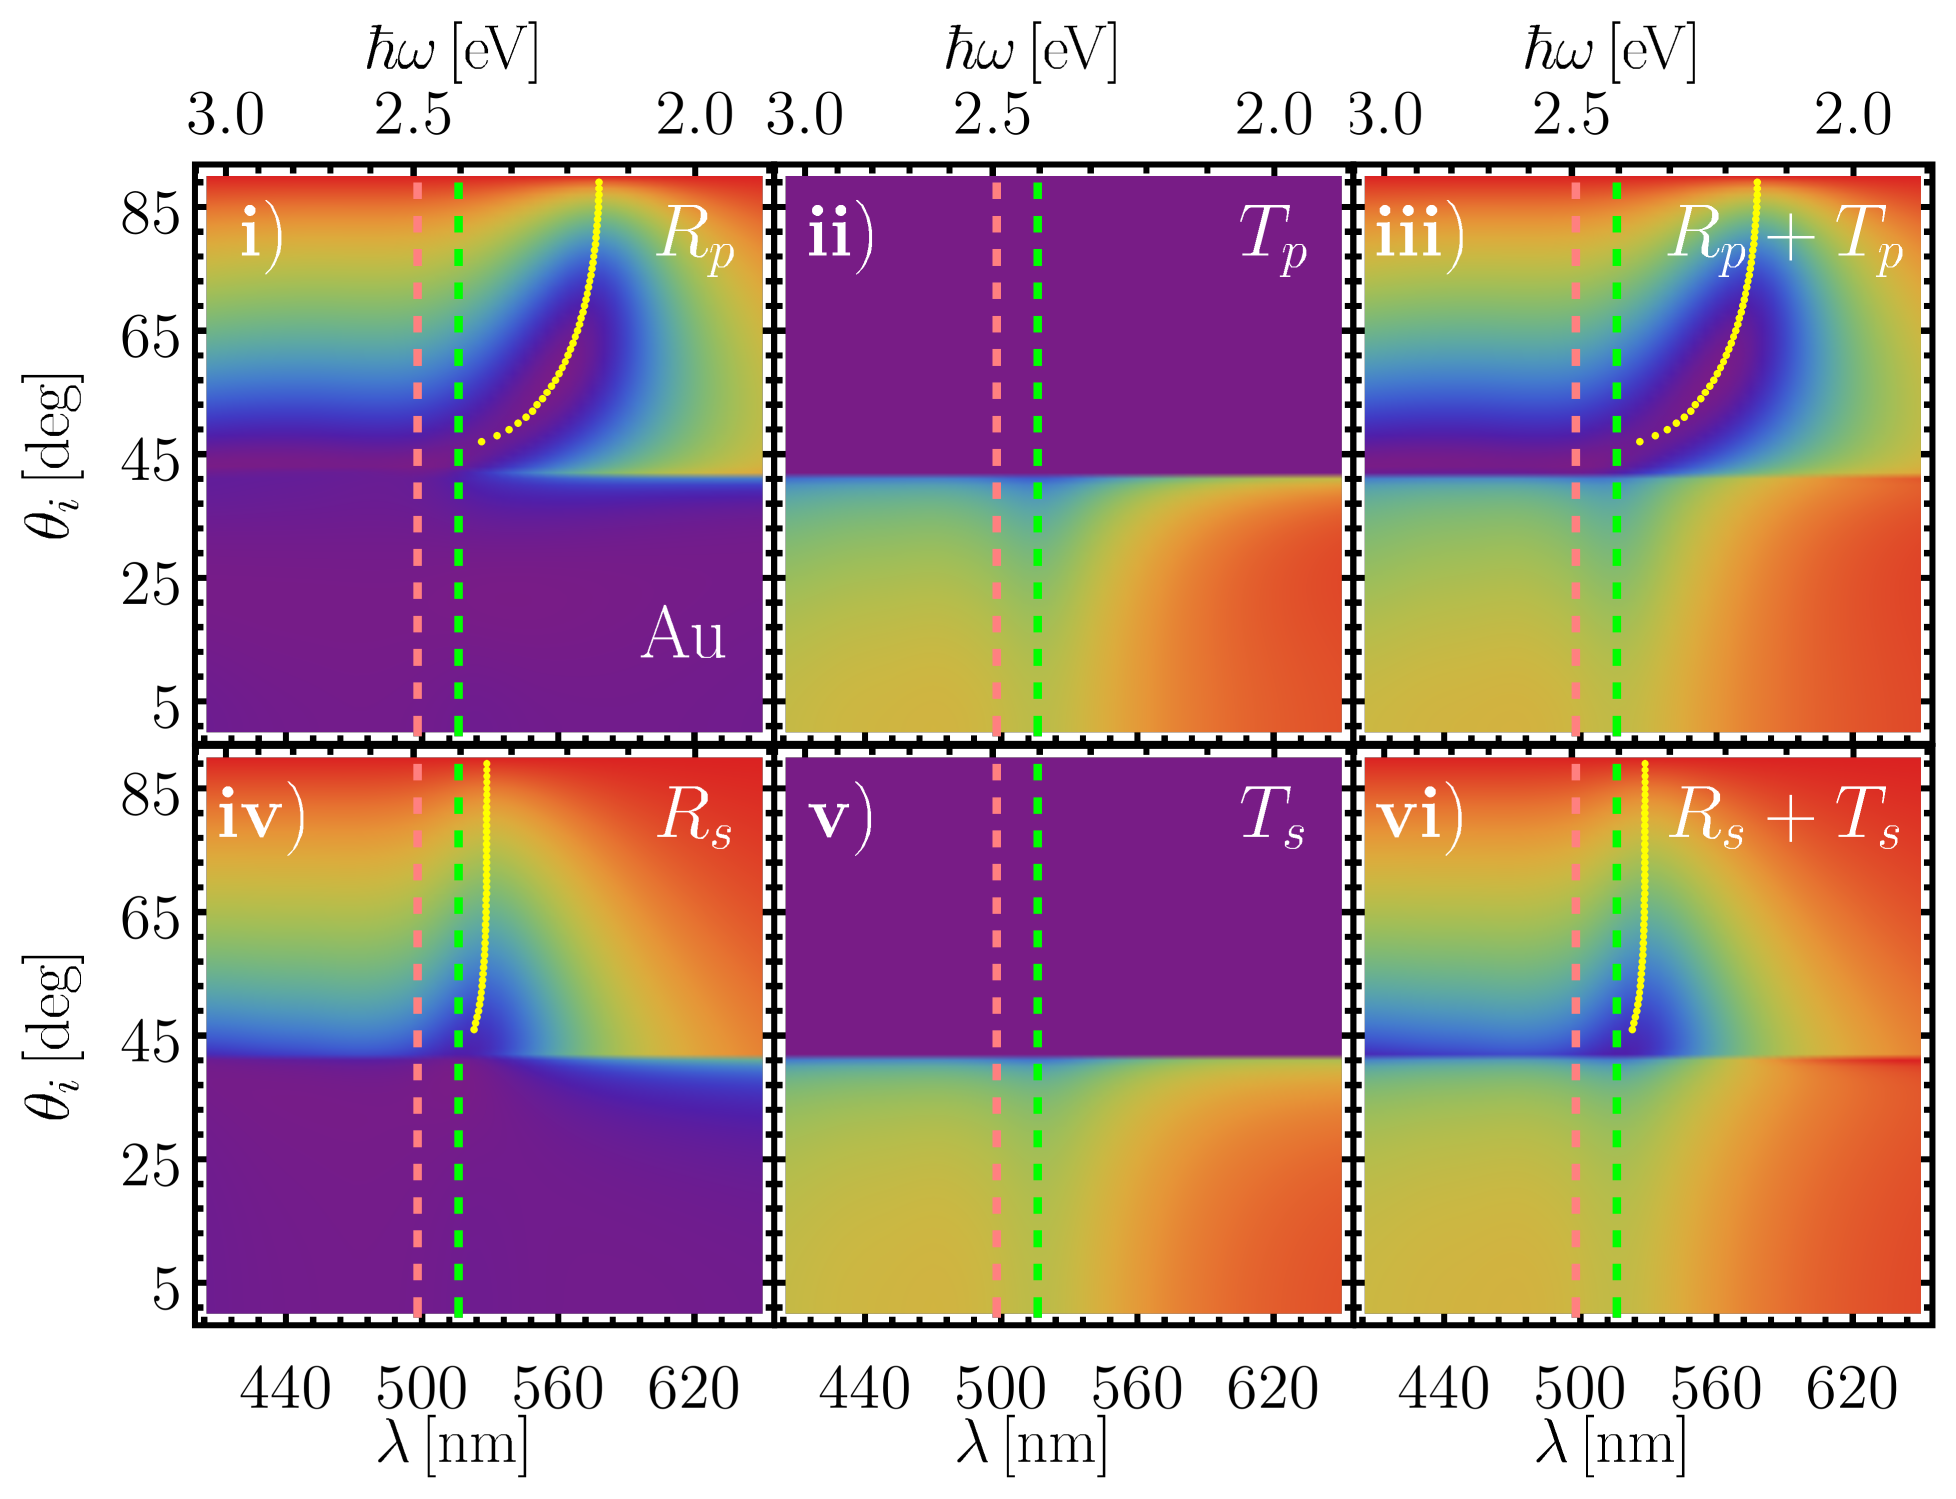
\includegraphics[scale=1]{2-Resultados/figs/10-RT-AuAg/0-2D_Grid_1.png}};
\node[right, inner sep=0pt] (legend) at (4.45,.15) {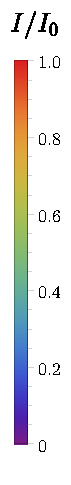
\includegraphics[scale=1, trim={00 -15 00 00}, clip]{2-Resultados/figs/0-IBar_v}};

\def\x{7.5}
	\node at(\x,1){\small NPs Au};
	\node at(\x,0) {\small $\Theta = 0.125$};
	\node at(\x,-1) {\small $a=30$ nm};

\def\xR{4.2}
\def\yR{2.5}	
	\node at(\xR,\yR){$R_p $};
	\node at(\xR,\yR-2.8){$R_s$};
\end{tikzpicture}	
	\end{subfigure}\\ \noindent \hspace*{-4em}
	\begin{subfigure}{.01\linewidth}\caption{}\label{sfig:RT-Ag}\vspace{5.5cm}\end{subfigure}\hspace*{-.5em}
	\begin{subfigure}{.7\linewidth}\hspace*{-.5em}
	\begin{tikzpicture}[scale=1]
\node[inner sep=0pt] (graf) at (.05,0){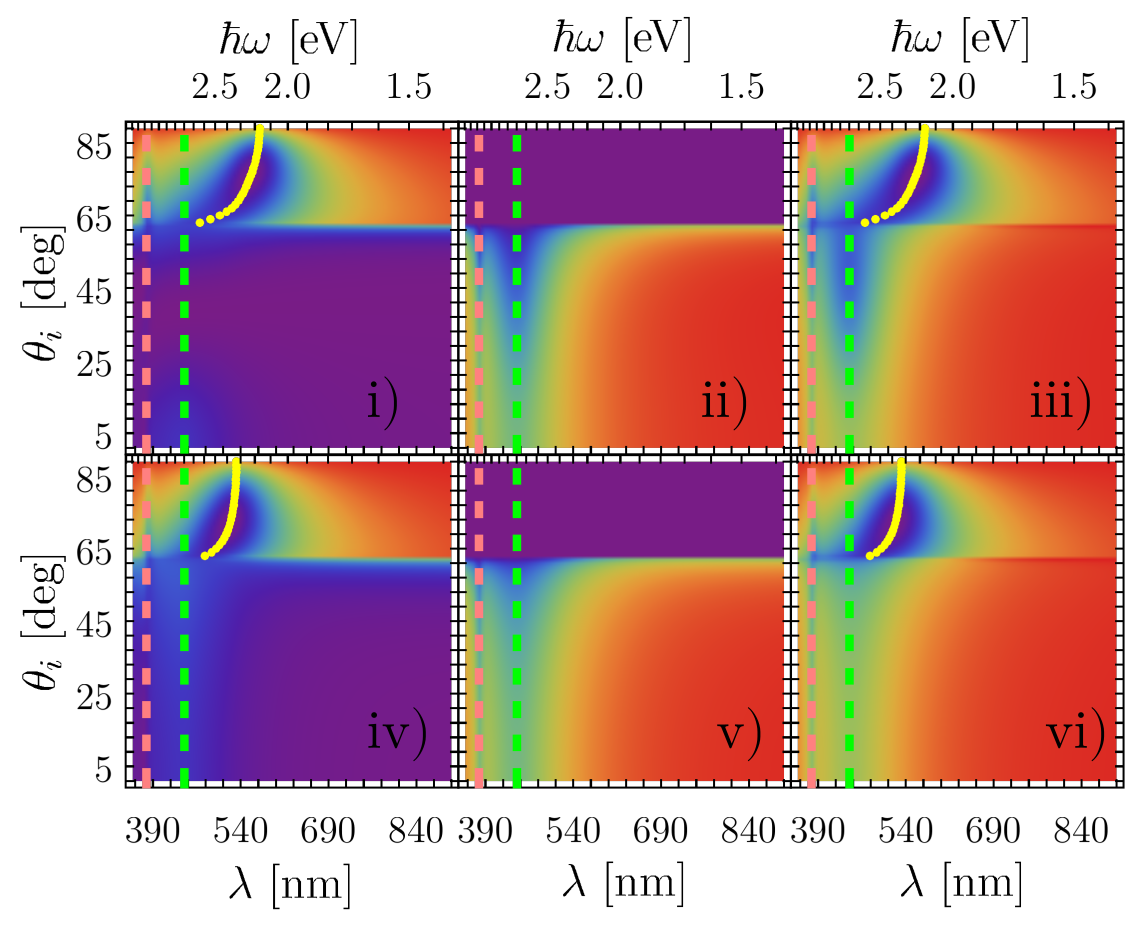
\includegraphics[scale=1]{2-Resultados/figs/10-RT-AuAg/0-2D_Grid_2.png}};
\node[right, inner sep=0pt] (legend) at (4.4,.15) {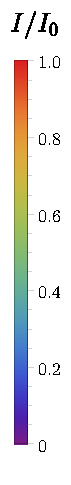
\includegraphics[scale=1, trim={00 -15 00 00}, clip]{2-Resultados/figs/0-IBar_v}};

\def\x{7.5}
	\node at(\x,1){\small NPs Ag};
	\node at(\x,0) {\small $\Theta = 0.1$};
	\node at(\x,-1) {\small $a=40$ nm};

\def\xR{4.2}
\def\yR{2.5}	
	\node at(\xR,\yR){$R_p $};
	\node at(\xR,\yR-2.8){$R_s$};
\end{tikzpicture}
		\end{subfigure}\vspace*{-.5em}
	\caption{Gráficas de la reflectancia $R$, transmitancia $T$ y la suma de éstas $R+T$   en configuración ATR de una monocapa de NPs esféricas como función del ángulo de incidencia $\theta_i$ y de la longitud de onda $\lambda$ (escala inferior) así como de la energía de la onda plana incidente en unidades de $\hbar\omega$ (escala superior), considerando \textbf{a)} NPs de oro de radio $a=30$ nm y fracción de cubierta $\Theta$ de $0.125$, y \textbf{b)} NPs de plata de radio $a=40$ nm y $\Theta=0.1$.  Las gráficas   en el renglón superior [\textbf{i)--iii)}]  muestran los resultados de la reflectancia para  polarización \emph{p} y las del renglón inferior  [\textbf{iv)--vi)}] para polarización  \emph{s}. Las líneas verticales punteadas verdes corresponden a la SP-SPRs dipolar ($\lambda\approx 531$ nm y $\lambda\approx 444$ nm para las NPs empleadas de oro y plata, respectivamente), y las rosas a la SP-SPR cuadrupolar ($\lambda\approx 514$ nm y $\lambda\approx 383$ nm para las NPs de oro y de plata, respectivamente). Los puntos amarillos corresponden a los mínimos en $R$, y $R+T$ para ángulos mayores a $\theta_c\approx 62.5^\circ$ y longitudes de onda mayores a la SP-SPRs dipolar. }\label{fig:RT-AuAg}
	\end{figure}	

El supuesto modo plasmónico colectivo, observado en una monocapa de NPs con una función dieléctrica tipo Drude, también aparece al considerar las funciones dieléctricas experimentales para el oro y la plata de \cite{johnson1972constants}, con sus respectivas correcciones por tamaño. Al considerar una monocapa de NPs de oro de radio $a=30$ nm con una fracción de cubierta $\Theta=0.125$ y una de NPs de plata de $a=40$ nm y $\Theta=0.1$ (ver Fig. \ref{fig:RT-AuAg}), es posible emplear el supuesto modo plasmónico colectivo para el sensado, considerando un intervalo para el ángulo de incidencia $70^\circ<\theta_i<80^\circ$ (ver Fig. \ref{fig:AuAg-Cuts-Rad-75}). Para evaluar el uso del supuesto modo plasmónico colectivo en el sensado, en la siguiente sección se estudia la respuesta del supuesto modo plasmónico colectivo ante cambios del índice de refracción de la matriz $n_m$ y, a su vez, se compara su respuesta con la de propuestas de sensores nanoestructurados basados en las resonancias de superficie localizadas \cite{svedendahl2009refractometric} y en las LSPRs \cite{danilov2018ultra}, así como con  biosensores plasmónicos comerciales, los cuales emplean la excitación del plasmón polaritón de superficie, excitados en una película continua de oro de $50$ nm \cite{estevez2014trends,svedendahl2009refractometric}.